\documentclass{sig-alternate}
\usepackage[utf8]{inputenc} 
%\usepackage[hidelinks]{hyperref}
%\usepackage[autostyle,french=guillemets,babel]{csquotes}
\usepackage{graphicx} % support the \includegraphics command and options
%\usepackage[backend=biber]{biblatex}
%\addbibresource{biblio.bib}
% \usepackage[parfill]{parskip} % Activate to begin paragraphs with an empty line rather than an indent
\usepackage{booktabs}
\usepackage{array}
\usepackage{paralist}
\usepackage{verbatim} 
\usepackage{amsfonts}
\usepackage{fancyhdr}
\usepackage{times}
%\pagestyle{fancy} % options: empty , plain , fancy
%\renewcommand{\headrulewidth}{0pt} % customise the layout...
%\lhead{}\chead{}\rhead{}
%\lfoot{}\cfoot{\thepage}\rfoot{}

\title{From Nested Virtualization Architecture \\To 2D Security Management for Distributed Clouds}

\author{
\numberofauthors{3}
\alignauthor
Alex Palesandro\\
\affaddr{Orange Labs, France}\\
\texttt{alex.palesandro@gmail.com}
\alignauthor
Aurélien Wailly\\
\affaddr{Orange Labs, France}\\
\texttt{aurelien.wailly@orange.com}
\alignauthor
Marc Lacoste\\
\affaddr{Orange Labs, France}
\texttt{marc.lacoste@orange.com}
}

\begin{document}
\maketitle

\abstract{
%Today, hypervisors have to find a complex trade-off between functionalities provided and security assurance. Those requirements are contrasting by design:
%adding new features will generally increases the LoC and consequently the attack surface. On the contrary, those code additions are required to properly fulfill market requests. 
%
%Nested virtualization is a technique capable to diversify hypervisor features. Exploiting an extra layer of virtualization, we will be able to decouple different requirements, avoiding the need to find delicate trade-off.
%
%In this paper, we will analyze the state of nested virtualization in modern hypervisor and evaulating the impact of utilization of microhypervisor to enforce a stronger security level.
%The problem of homogeneity over multiple IaaS providers is receiving considerable attention with the evolution toward nested virtualization. These new architectures unveil user-centric opportunities such as efficient resources management and VM migration. However the inherent drawbacks hinder its global adoption with a larger TCB and the complexity to monitor another virtualization layer. Thus, we argue that the promising architectural view of micro hypervisors approach is the key to the separation of hypervisor duties and reducing the attack surface.
%
%Furthermore, our architecture mushrooms commodity and micro hypervisors to leverage nested virtualization in terms of user-data privacy, modularity, TCB size and compatibility. These design principles are evaluated for each architecture configuration and compared to establish a reference security architecture. The resulting combination is built over common hypervisors empowered with micro hypervisors features. A reference implementation proven the architecture to be viable and will be extended to meet broader hypervisor scopes, enabling migration over heterogeneous cloud servers.
Distributed cloud computing is now moving user-centric. The pro-mise of this evolution is: (1) unified resource management across IaaS providers, e.g., live migration independent from hypervisor technology; (2) increased customizability to choose the hypervisor services needed to realize fully à la carte, self-service clouds. However, a reality check shows that major interoperability and security barriers must be lifted, and complex trade-offs be found between functionalities provided and security assurance.
Nested virtualization (NV) brings both a homogeneous interface for distributed hypervisor features and enhanced IaaS security, protecting VMs even in case of hypervisor compromise. However, practical NV adoption is still hindered by code additions to an already very large hypervisor TCB and by limited hardware support. New distributed IaaS architectures are therefore required.\\

In this paper, we argue that micro-hypervisor (MH) architectures are the key to overcome such NV limitations. 
From the previous challenges, we derive a set of design principles that a distributed IaaS architecture should satisfy. 
We compare possible architectural designs combining NV with micro-hypervisor features to find the best trade-off between user data privacy, modularity, TCB size, and compatibility with multiple platforms. 
We sketch how the resulting architecture may serve as a basis for 2D security management of a cloud of clouds: vertically, across layers for hardened IaaS security, and horizontally spanning cloud domains for end-to-end security.
}

%The first challenge means that threats will be both vertical, spanning layers, and horizontal, spanning domains  the SUPERCLOUD being a multi-layer, multi-domain distributed cloud infrastructure. Vertically, attacks currently target several infrastructure layers (e.g., VMs, hypervisor). Unfortunately, most existing defenses are generally for single layers only. This makes it difficult to grasp the overall extent of an attack. Horizontally, threats may propagate through the network from cloud to cloud. Unfortunately, most existing defenses are for single clouds only. Lack of interoperability in security policies and mechanisms is thus a major barrier to  unified hybrid cloud security. The second challenge means that although many defense mechanisms may be leveraged in this 2D landscape, they remain difficult to configure and to reconcile. The current “by hand” approach becomes a nightmare for security administrators. Despite some automated solutions for managing security of single clouds, there is currently no solution truly applicable to federations of clouds in practice.



%The resulting combination is built over common hypervisors empowered with micro hypervisors features. 
%
%rchitecture mushrooms commodity and micro hypervisors to leverage nested virtualization
%
%
%
%Furthermore, our architecture mushrooms commodity and micro hypervisors to leverage nested virtualization in terms of user-data privacy, modularity, TCB size and compatibility. These design principles are evaluated for each architecture configuration and compared to establish a reference security architecture. 
%
%enhance NV architecture next generation of distributed clouds security and interoperabiltiyi issues.
%
%
%failureverall, current NV architectures lack some of the dedicated features found in modern hypervisors and the impossibility to rely on a tiny TCB (violating principles DP3 and DP4).
%If the first one is currently being addressed by hypervisor developers, the second simply has not be achieved with modern hypervisors so far.
%
%ypervisors have to find a complex trade-off between functionalities provided and security assurance. Those requirements are contrasting by design:
%%adding new features will generally increases the LoC and consequently the attack surface. On the contrary, those code additions are required to properly fulfill market requests. 
%
%the inherent drawbacks hinder its global adoption with a larger TCB and the complexity to monitor another virtualization layer.
%
%First, independence from the provider resulting in lower infrastructure operation overheads, more rapid deployment of services, but also increased homogeneity the customer being free a particular hypervisor technology. Second, increased customizability, as the customer can choose which virtualized services (e.g., for security) may be deployed resulting in fully a la carte clouds. Third, new business opportunities, as SCs and their (virtual) apps might become new markets in the manner of ecosystems from the mobile computing world (e.g., iPhone, Android). 
%
%User-centric: de DCC
%vers plus d'homogeneity
%problemes 
%verticaux
%horizontaux.
%
%NV: solutions pour résoudre certains de ces problèmes.
%
%VErticaux: ...
%Horizontaux: ...
%
%Mais limites ... + ...
%New architectural solutions must be found.
%
%In this paper explore potential of micro-hypervisor architectures to enhance NV architecture next generation of distributed clouds security and interoperabiltiyi issues.
%
%We explore design principles properties.
%
%We compare architecutral solutions combining NV+MH to find the best trade off between ..., ???; ... meilleure approche.
%
%We sketch finally: how this type of architecture could enable to perform 2D supervision xl alyer x domain.


\section{Introduction}
\label{sec:intro}

%% Motivation
%Cloud computing platform are a solid reality nowadays. 
\noindent Distributed cloud computing is now becoming a reality. Modern cloud platforms are able to provide elastic use of resources, optimizing their allocation to meet user needs. However, currently deployed distributed cloud infrastructures present several limitations.

% Interop
DCC does not handle heterogeneous infrastructures which secludes providers in non-evolving hardware.
% Securite
Also, security remains the last hurdle toward wide adoption of DCC. The user data are no more self contained but distributed among all parties without any proof of confidentiality, integrity or availability.

%% Specific problem considered
We classified problems related to DCC horizontally and vertically. The horizontal view gathers features related to interactions between IaaS stacks, such as live migrations. The vertical view addresses features close to the isolation of execution environment on the same physical machine. This classification provide a global coverage of problems to solve to deliver a secure, stable and robust architecture.

%% "In this paper we show that"
As a first element of answer, the nested virtualization~\cite{turtle:ibm} performed a breakthrough with enhanced isolation capabilities on the same physical machine. The hypervisor is now virtualized by a thin layer~\cite{cloudvisor:zhang} to counter failures. Furthermore, the horizontal challenges were also included in this tiny layer to deliver an homogeneous interface for commodity hypervisors~\cite{art:blan, xclo:blank}. However these classic approaches suffers from several shortcomings detailed in Section~\ref{ref:challenges}. Thus we propose a novel architectural approach to undertake remaining problems.

%% Differences with others
The previous works created both horizontal and vertical basic blocks from scratch. While being a necessary step, these approaches does not inherits the advances performed in terms of operating system security. The software architecture are mainly monolithic and yet-another-layer fends off security problems without
figuring them out. Our approach learns from security issues fixed by OS architecure~\cite{} and apply these patterns to leverage nested virtualization. In this paper we show that component-based architecures are a promising design for the next generation of clouds.

This paper is organized as follows. Section~\ref{ref:challenges} details the constraints of nested virtualization for the two dimension of our solution. In Section~\ref{sec:rw} we analyze the nested virtualization ecosystem and position existing solutions regarding our design principles. In Section~\ref{sec:classic}, we details limitations of classical nested virtualization approach and in Section~\ref{sec:mh} we present the microvisor approach. In Section~\ref{sec:archcomp} we compare cloud architectures propositions, combining nested virtualization and microvisors, leveraging the design principles grid introduced before.
%Furthermore, in Section 6 we define a security architecture for multi-cloud scenario, with an analysis of necessary software components to satisfy vertical design principles.
In Section~\ref{sec:conclu}, we conclude the paper with future works and our vision of the SuperCloud.
% in section in section 6 we define a security architecture for multi-cloud scenario, with an analysis of necessary software components to satisfy vertical design principles. In section 8, we conclude the paper with future works in section 8.

\section{Challenges and Design Principles}
\label{ref:challenges}

First, deploying cloud applications able to transparently leverage resources of several heterogeneous platforms is still difficult. The concept of super-cloud~\cite{art:blan, xclo:blank} tries notably to overcome such issues. Multi-platform coordination is hard, primarily due to lock-in to different standards such as VM formats. Unfortunately, such lock-in is not only due to market strategic decisions, but also reflects heterogeneity of virtualization technologies. For example, each cloud provider may use different storage systems or different formats to store VMs images. Different hypervisors have nowadays a low degree of compatibility between them. This generally prevents leveraging some popular features like VM live migration between different platforms. Incompatibility is even greater if we consider that each platform may adopt several types of virtualization techniques. This situation induces a tight dependency between the customer and the cloud provider. It may prevent guaranteeing service availability by relying on alternative providers, or to set up geographical optimizations due to cost or origin of traffic. This has resulted in some dramatic data server failures in recent years, causing prolonged outage of service for many applications. In what follows, we refer to this class of multi-platform issues as \textit{horizontal} challenges.

Second, a number of issues have been raised about user data privacy and platform integrity. From the user perspective, users would like to preserve privacy of their data stored on the cloud platform. However, due to overprivileged hypervisors, a curious or malicious administrator could easily retrieve such data~\cite{cloudvisor:zhang}. In a multi-tenant cloud platform, physical resource sharing between users may lead not only to data leakage or but also attacks against the IaaS~\cite{bot:att, sec:you}.
From the provider perspective, a key objective is to thus guarantee platform integrity against rogue VMs. However, commodity general-purpose hypervisors (GPHs) make it difficult to observe deeply all layers of a running IaaS platform. Indeed, running GPHs at the highest level of privilege hampers detection and reaction on the hypervisor itself in presence of faulty or malicious behavior -- unless to cause interruption of service for all hosted VMs. Thus, both user-centric and provider-centric visions of the cloud have a problem with overprivileged hypervisors.
%: the platform administrator cannot perform in-depth infrastructure monitoring nor can users concretely inspect administrator actions on their data. 
A major challenge for new generations of cloud infrastructures is thus to find acceptable trade-offs between such conflicting requirements. In what follows, we refer to this class of layer-oriented issues as \textit{vertical} challenges.

We identified five key design principles (DP) that a IaaS architecture should implement to meet the previous challenges. In what follows, those principles will serve as reading template to analyze different architectures.
\begin{itemize}[]
\item \textbf{DP1 User Data Privacy} A curious or malicious administrator (or another platform user) should not be authorized to inspect and analyze user data and VM instances without explicit user consent relying on mutually trusted services. A trade-off should be found to allow providers to detect and react to potential threats, but also to prevent unlimited platform and user data access in such inappropriate operator behaviors. Thus, a platform administrator should not manage the infrastructure directly using the highest level of privilege. Instead, his actions on user data objects should be validated by a mutually-trusted kernel run in the most privileged mode. This kernel should also enforce memory page encryption to prevent snooping when pages are swapped out.
\item \textbf{DP2 Fail-Safe Modular Architecture} The architecture should be fail-safe: for instance, to enable automatically migration of instances or user-data in presence of a threat and to recover from software failures. To reach this goal, the amount of safety-critical components should be as low as possible to mimize the attack surface. Similarly, the overall design should be as modular as possible to enable platform reconfiguration.
\item \textbf{DP3 Small TCB} The number of potential failures and bugs in the platform is directly linked with the code size executed at the highest level of privilege. Thus, an architecture with a tiny TCB (Trusted Computing Base) will improve safety and integrity by design.
\item \textbf{DP4 Inter-Platform Support} The cloud architecture should allow supporting directly different platforms and service providers. The same user virtual instances should be allowed to be run (and potentially migrated) unmodified over different IaaS platforms.
\item \textbf{DP5 Compatibility with Legacy} Evolution in the IaaS architecture should avoiding disrupting existing third party applications. Thus, platform interfaces should be kept as close as possible to existing ones, to prevent code rewriting notably for applications.
\end{itemize}
In addition to the above functional design principles that specify which features have to be achieved by the platform architecture, another set of non-design principles (NDP) should be considered regarding effective feasibility of implementing the architecture. We just give an example in terms of platform usability:
\begin{itemize}[]
\item \textbf{NDP1 Minimal Additional Code} A major issue could be represented by the amount of code to be added and maintained to an existing architecture to meet functional requirements. Despite not being a strictly a technical limitation of the architecture, it could become a show-stopper to its practical use.
\end{itemize}
In our analysis, we will consider not only the overall suitability of the architecture, but also the amount of effort needed to develop and deploy it. Table \ref{int:des} summarizes the previous principles and which class of requirements they address.
 
\begin{table}
\caption{Design Principles for a Distributed IaaS Platform.\label{int:des}}
\begin{tabular}{lll}
\toprule
\textbf{Id} & \textbf{Design Principle} & \textbf{Class of Requirement} \\
\midrule
DP1 & User Data Privacy & Vertical \\
DP2 & Fail-Safe Modular Architecture & Vertical \\ 
DP3 & Small TCB & Vertical \\
DP4 & Inter-Platform Support & Horizontal \\
DP5 & Compatibility with Legacy & Horizontal \\
NDP1 & Minimal Additional Code & -- \\
\bottomrule
\end{tabular}
\end{table}
 
\section{Related Work}
\label{sec:rw}

% Intro + performance issues
Several works presented in literature integrates these a subset of this design principles in their architecture, leveraging nested virtualization \cite{turtle:ibm,art:blan, cloudvisor:zhang}
Cloud computing feature set could be enlarged exploiting two layers of virtualization instead of just one. The presence of two different hypervisors allows the possibility to specialize hypervisors functions. Instead of having a general purpose hypervisor we could split the hypervisor role in two different layers, interconnected with a well defined interface.
Each layer will have to care about a subset of features, simplifying overall development.
However, nested virtualization on x86 architecture faced impeding performance issues \cite{rec:virt}.

% Perfomance issuess adressed
However, several works demonstrate that it is possible to put in place low overhead nested virtualization using special approaches \cite{turtle:ibm} . Moreover, other works try to recover performance loss exploiting multi-level consolidation, introduced in nested virtualization \cite{art:blan}. In conclusion, nested virtualization slowdown could be considered nowadays an acceptable price to achieve advanced features and, in addition, hardware manifacturers are developing and proposing new hardware facilities to reduce this overhead \cite{vmcs:nakajima}.

To sum up, no architecture had been presented to address vertical and horizontal class of problems at the same time until now. XenBlanket does not investigate cloud architectural security concerns (DP3,DP2), limiting the focus on new potential feature of a coordinated multi-provider cloud. Cloudvisor proposed a security architecture that leverages nested virtualization without allowing the possibility of executing more than one nested hypervisor at time, that is a crucial requirements of a multi-provider cloud platform (DP4). In a SuperCloud scenario, each user has to run its own L1 hypervisor instance to enforce a compatibility layer, overcoming incompatibilities between different providers.

Other approaches leveraging only one layer of virtualization does not achieve the whole design-principle satisfaction. Self-service cloud approach (SSC) \cite{ssc:art} design a complete security architecture to overcome major security and privacy issues of currently deployed cloud infrastructures, in order to alleviate the different needing user-centric and provider-centric vision of cloud computing presented in \ref{sec:intro}. Even if this architecture reproduces an approach similar to the SuperCloud without leveraging an extra layer of virtualization (DP4), the approach changes the behavior where the user acts introducing new components that have to be directly managed by the user. Therefore, the main drawback of this solution is to change the interface with the user, preventing the possibility to straightforwardly move to the new platform without having to change its applications (DP5).

% Integration NDSS Taming
Furthermore, DeHype \cite{wu2013TamHosHypMosDepExe} presented a dissected version of KVM hypervisor, trying to reduce the TCB of this popular hypervisor. The approach consisted in demoting a great part of the hypervisor codebase to a user-level execution. DeHype satisfies all vertical design principles listed before (DS1,DS2,DS3), reinterpreting the microkernel approach defining  the greatest part of code to userspace. DeHype increases a lot the robustness of a cloud platform leveraging KVM, limiting for example the possibility of attack in multi-tenancy platform, but it does not address horizontal design principles about a multi-provider service.

\section{Current Nested Virtualization}
\label{sec:classic}

\subsection{Principle}

\noindent \textit{Nested virtualization (NV)} refers to a system architecture with two layers of virtualization~\cite{turtle:ibm}. It consists in ``virtualized'' virtualization: the guest system virtualizes a nested guest. The concept may be generalized to an arbitrary number of nested guest layers, leading to recursive virtualization~\cite{rec:virt,Popek:1974:FRV:361011.361073}. (Full) virtualization is able to execute tasks in a deprivileged context that normally requires a privileged execution. With NV, this approach may be extended to virtualization itself: a guest hypervisor may be run with nested guest VMs without requiring any change to any of them.
%More formally, Popek \& Golberg \cite{Popek:1974:FRV:361011.361073} discussed this subject, introducing the concept of ``recursively virtualizable'' machine and giving an initial definition of recursive virtual machines: If it is possible for a virtual machine to run under itself a copy of the VMM that could also exhibit all the properties of the VMM and this procedure could be repeated until the resources of the systems are consumed, then the original machine is recursively virtualizable.

Two layers should be distinguished when migrating to an NV architecture: (1) the hypervisor running above the hardware (\textit{L0 hypervisor}); and (2) the nested hypervisor (\textit{L1 hypervisor}). Nested guests are generally referred to as \textit{L2 guests}.
Unfortunately, virtualization comes with a price due to the extra layer of indirection introduced: the computational overhead is generally acceptable when dealing with single-layer virtualization, but grows exponentially when adding further levels~\cite{rec:virt}. This huge performance overhead prevented NV adoption during many years. However, Ben Yehuda et al. finally proposed an architecture tending towards more reasonable overheads~\cite{turtle:ibm}.

NV feasibility opened plenty of new possibilities and avenues for research that have been largely discussed in the literature~\cite{turtle:ibm,rec:virt,art:blan}. Such works all tend to diversify hypervisor functionalities, introducing new features but also keeping existing ones. It turns out that each layer addresses clearly different sets of issues.

L0 tackles vertical aspects of the platform. It aims to guarantee the best performance and strongest level of isolation possible. L0 represents the last line of defense of the platform and a privileged point for monitoring of its global status.

L1 is responsible for horizontal feature set. It has to provide the widest possible support for different platforms and the ability to virtualize using different techniques e.g., para-virtualization, hardware-assisted virtualization, dynamic binary translation. {\sffamily To address such requirements, Williams et al.~\cite{art:blan} proposed a patched version of Xen, Xen Blanket, to realize an L1 virtualization layer designed to run over different hypervisors. This notably enables to run and to perform live migration of the same VM over different physical cloud infrastructures.} % A migrer dans le related work?

\subsection{Limitations}

\noindent Today, NV presents several limitations related to hardware support {\sffamily and software state of implementation}. 

First, to support NV, the hypervisor has to provide an exact copy of hardware virtualization primitives. Full virtualization with hardware assistance (HAV) is the most popular technique, but requires quite a complex dedicated support.
HAV primitives assist instruction emulation, memory address translation, and management of devices. Both Xen and KVM propose {\sffamily nested VMX/SVN features} that allow to efficiently handle nested hardware virtualization on single-layer hardware primitives.
Full virtualization is currently the only virtualization technique supported for L1 virtualization due to its ability to run unmodified guest OSes -- and thus hypervisors. Paravirtualization (PV) would on the contrary require an ad hoc modified hypervisor to act as L1 (thus violating the NDP1 principle).
%To address this performance problems, several hardware producers proposed new facilities, like Intel VMCS shadowing, that reduces the amount of nested VMEXIT when handling a nested guest VMEXIT.
Despite still poor NV performance and not being yet stable on modern hypervisors~\cite{xen:test}, such feature is under heavy development and will hopefully be in a usable state soon.

Second, due to current monolithic GPH architectures, each feature directly introduced within the hypervisor such as security enhancements enlarges the TCB~\cite{cloudvisor:zhang}. Therefore, a huge amount of code runs in highly privileged mode and must be trusted. Several works discuss and analyze the overall TCB of modern GPHs, always bigger than 100 KLoC~\cite{nova, xmhf}. This approach directly violates the DP3 design principle.
%that identified a small TCB as a major requirement for a solid architecture.
%A brief comparison of TCB of widespread GPH is depicted in figure \ref{fig:tcbchart}. 
%More importanly, this is particularly true looking at the monolithic approach of commercial hyper-visors, where any addition to the hypervisor body enlarges the TCB.
Moreover, the previous architecture does not improve overall stability of the infrastructure. The bottom-most hypervisor L0 faces the same issues as single-layer GPH architectures: a large TCB implies also that a failure experienced in one of its critical components may trigger a generalized failure of the whole platform (violating the DP2 principle). Besides, in standard GPH architectures, the administrator has the entire control of the platform and could potentially snoop and inspect user VM status and data (violating the DP1 principle).
Such designs notably do not take advantage of the possibility {\sffamily to use a platform compatibility layer}, and more modular architectures with only a tiny security-critical kernel.

Overall, current NV architectures lack some of the dedicated features found in modern hypervisors and the impossibility to rely on a tiny TCB (violating principles DP3 and DP4).
If the first one is currently being addressed by hypervisor developers, the second simply has not be achieved with modern hypervisors so far.

\section{Micro-Hypervisors}
\label{sec:mh}

%\begin{figure}
%\caption{GPH TCB comparison \cite{nova}}
%\label{fig:tcbchart} 
%\begin{center}
%\includegraphics[width=\columnwidth]{figures/TCBchart.png}
%\end{center}
%\end{figure}

% Xen and KVM TCB

\subsection{Principle}

\noindent To solve the TCB size issue, several works have introduced the idea of \textit{micro-hypervisor (MH)} architecture~\cite{nova, NoHype, xmhf}. To reduce the hypervisor size, such new hypervisor architectures draw inspiration from evolution in OS architecture (e.g., extensible, micro-, exo-, component-based kernels). Within the hypervisor are distinguished security-critical modules from non-sensitive code. The aim is to expel as much code as possible from the TCB and target ultra-thin hypervisors. For instance, some components of the hypervisor (e.g., device drivers, VM address space management) may be virtualized outside the micro-hypervisor, isolated, and restarted in case of compromise~\cite{nova}. The extreme case is to remove the virtualization layer altogether~\cite{NoHype}.

with a traditional microkernel-like design that tries to consistently reduce the amount of code running with the highest privilege level. 

A micro-kernel traditionally consists in a minimal kernel running in privileged mode, offering only a few fundamental services to other modules (e.g, scheduling, IPC, memory management) running in a less privileged domain. All other components, such as device drivers, are moved out in user-space. While the benefits of such a design has been questioned due to the cost of IPCs in first generations of micro-kernels, such arguments have since then been completely dispelled~\cite{liedtke1993ImpIPCbyKerDes,liedtke1995micConnova}.
%Microkernels had been questioned because of the wasteful performance of first generations, due to IPC intrinsic cost. This argument had been completed confuted by Liedtke in 1993: \cite{liedtke1993ImpIPCbyKerDes,liedtke1995micCon}.

%Architectural solutions were also created to make the hypervisor more minimal and flexible, targetting its two most vulnerable elements: (1) the core hypervisor itself; and (2) the management VM (e.g., Xen Dom0).
%
%A first class of solutions aims \textit{to reduce the hypervisor size}. The new hypervisor architecture should be more minimal, drawing inspiration from evolution in OS architecture (e.g., extensible, micro-, exo-, component-based kernels). Within the hypervisor are distinghuished security-critical modules from non-sensitive code. The aim is to expel as much code as possible from the TCB and target ultra-thin hypervisors, also known as \textit{micro-hypervisors}. For instance, some components of the hypervisor (e.g., device drivers, VM address space management) may be virtualized outside the micro-hypervisor, isolated, and restarted in case of compromise~\cite{NOVA}. The extreme case is to remove the virtualization layer altogether~\cite{NoHype}.
%Unfortunately, although promising, such architectures usually require extensive code rewriting. They also provide a very limited number of resource management services unlike an operational IaaS infrastructure. They are thus hard to apply to mainstream hypervisors today.
One of the benefits of micro-kernels is to enable to easily redesign a hierarchy of privileges. A user application normally trusts the micro-kernel and only the set of user-space services it requires. However, such drivers and libraries may not be trusted by every application run on the system. User applications share the system but may need to support completely different set of system services. This allows micro-kernels to implement different ``personalities''. However, the interest of such ``personalities'' has been largely reduced by the fact that system services, device drivers and even applications have to be completely re-designed to fit this new architectural pattern. Therefore, with the introduction of VMs, microkernels lost the battle in favor of hypervisors, in terms of popularity. However, the great advantage of tiny TCB, provided by microkernel, was not provided also by hypervisors. As we analyzed before, they present normally a monolithic architecture, like the great part of modern OS. This feature kept alive the interest in microkernels, in particular trying to couple microkernel benefits with virtualization\cite{Heiser}.

Therefore, leveraging this concept of microkernels, a micro hypervisor (MH) is composed from a small kernel providing only essential functions, like scheduling, IPC, memory management and VMX extension. Several micro-hypervisor have been proposed in literature \cite{xmhf, nova}. They rely on the micro-kernel paradigm, extending it to virtualization. MH naturally satisfy vertical design principles (DP1,DP3, DP4). The tiny core could be considered the only system-critical componente of the architecture and, due to its relative small dimension and the consequent minor attitude to vulnerabilities,it could represent the ``last line of defense''.

In addition, MH inherits the concept of micro-kernel to implement different ``personalities''. Those ``personalities'' are concretely a set of ``processes'' handling specific functions running in user-space. As those functions are implemented outside the kernel, each user could rely on a different instances of the hypervisor user-space process, that could coexist at the same time. This process separation between user could enforce a straightforward mechanism to neutralize VM-to-VM attack from a malicious user. Moreover, user-space processes are easier to debug with commodity tools (GDB, valgrind).
Finally, this extraction process drives to a more solid platform, considering that user-space crashes are generally not fatal for the entire system integrity.  A possible example, that will be analyzed in next section, is the user-space VMM component of Nova, Vancouver, that resides in user-space \cite{nova}.
In addition, this approach is not far from the one proposed in DeHype \cite{wu2013TamHosHypMosDepExe}, where a consistent part of the KVM hypervisor has been demoted in user-space.

\subsection {Limitations}

Despite the positives, MH approaches had demonstrated some limitations. Firstly, the straightforward one is the initial lack of hardware support, lack of device drivers are still a relevant Achilles' heel for this solutions, inherited from its ancestors microkernels. Fortunately, this kind of issue could be addressed leveraging I/O passthrough techniques, although it will cause exclusive allocation issues.

Moreover, as reported in previous sections, several cloud computing issues are simply not addressable with general purpose hypervisor (GPH). However, they are commonly widely adopted and represent the bedrock of existing platform. Therefore, GPH exports wide and solid interfaces leveraged by a plenty of different software that is able to properly communicate and act through them on the virtualization layer. On the contrary, MH lack of cloud toolkit integration, requiring an explicit support to be written, not satysfing 3rd part compatibility requirements (DP5). GPH are tightly connected with cloud toolkit and could present solid interfaces to communicate with different tools. 

Finally, microkernel modularization introduce a major challenge in architecture design. Due the increased complexity, for sake of kernel size, MH could generally lack of several virtualization features, commonly available on modern GPH hypervisor. For instance, XMHF does not support multiple guests. This kind of drawbacks could limits the potential interest in MH, even they are able to introduce several important features.

\section{Architecture Comparison}
\label{sec:archcomp}

\begin{figure*}
\begin{center}
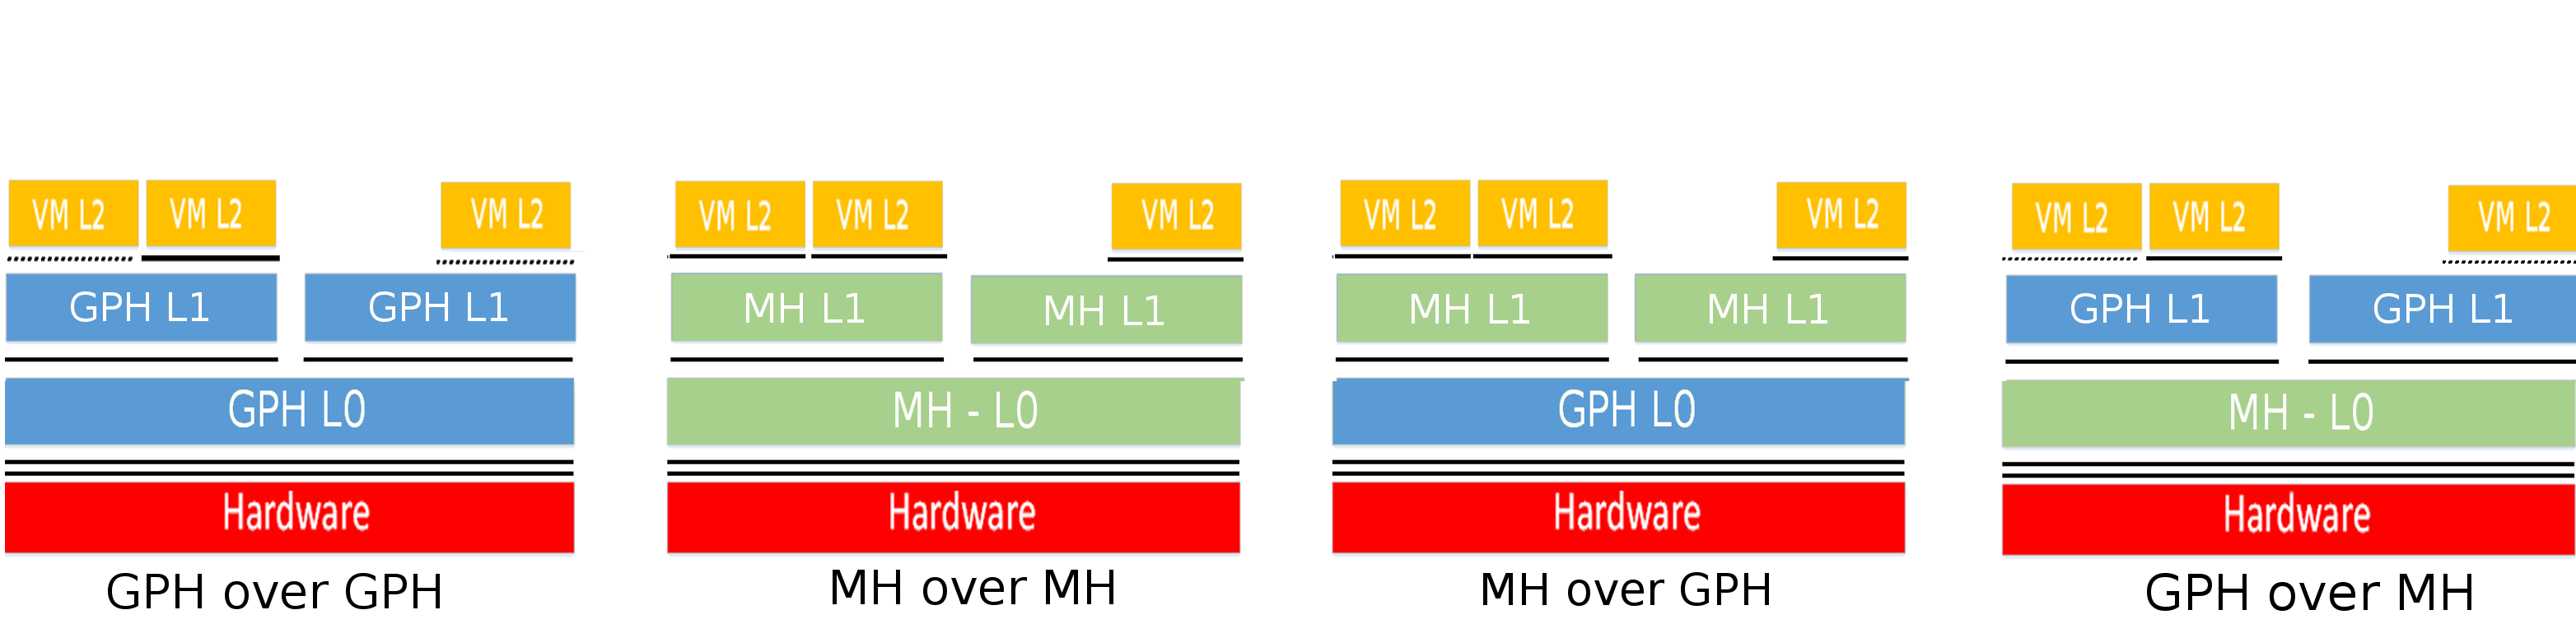
\includegraphics[width=2\columnwidth]{globalcut.png}
\end{center}
\caption{}
\label{fig:io}
\end{figure*}

\noindent The adoption of an extra layer of virtualization is capable to introduce a remarkable set of new features but it does not reduce the dimension of Trusted Code Base (TCB).
MH could represent a new approach to improve the potential benefits provided by the adoption of nested virtualization. In the following subsections, it will presented the four possible architectures achievable ``nesting'' of GPH and MH, underlying potentialities, drawbacks and potential cost of implementation.

\subsection{GPH Over GPH}

The first analyzed architecture concerns only GPH. At first, it is important to recall the most interesting achievable by such architectures. In particular, several remarkable features are live migration over different platform, transparent migration of virtualized clusters between different data-centers (horizontal requirements DP1).
Supposing the completeness and the correctness of nested virtualization hardware facilities in widespread hypervisor, GPH over GPH satisfies all horizontal design principles, but it lacks in vertical DPs as the size of TCB is the same of currently deployed architectures.

To sum up, it could be possible to achieve live-migration between different platform and other features related to VM management flexibility but it could not still be possible to reduce the TCB. Analyzing MH approaches, the aim is try at most to retain to features, trying to introduce isolation and privacy improvements due to the lower TCB promised.

%Although this architectures presents an extra layer between the nested guest, normally controlled by the cloud user and the system critical part, L0, the latter is far from a satisfying security level. The TCB of KVM that is represented by the entire Linux Kernel is normally around 200 KLoCs, considering the medium size of a deployed Linux kernel.
%Moreover, default KVM configuration does not provide a transparent protection mechanism between different VMs, so that compromising one instance of QEMU, that is executed in user-space, an attacker could compromise all the others VMs on the platform.

\subsection{MH Over MH}

MH on MH in reported only to see the orthogonality between this approach and GPH over GPH.
A theoretical implementation of MH over MH will provide the vertical requirements that are missing in the previous approach. The tiny core could be able to overcome monolithic problems due to privilege level of administration tasks (DP1), the possibility to improve the resilience of the platform to a large set of software failures (DP2) and finally reduce the possibility of the vulnerabilities of the most privilege part of the software (DP3). However, the interest on such architecture is limited because it is not able to overcome any cited issues of single-layer MH. Moreover, several horizontal properties are theoretically achievable but they will require a huge effort in developing functions of interest. Moreover, the lack of nested VMX functionalities prevents to concretely test this kind of architecture, because MH normally rely on VMX facilities in order to create a nested HVM guests.
To conclude, nested virtualization is exploited in order to fill eco-systems gaps with GPH but MH over MH does not provide any improvement in this sense.

\subsection{MH Over GPH}
\label{par:mog}

The third architecture, proposed in order to reduce security concerns, is built combining an GPH at L0 and a MH at L1. 
%Several MH are proposed in literature focusing on different .
%Therefore, this model tries to exploit microhypervisor as L1 hypervisor in order to enforce better isolation between L2 and L0. L1 will exploit the emulated nested VMX provided by GPH L0 and virtualize L2. 
%With this approach, we try to isolate the attacker in a VM virtualized on a secured layer, in order to prevent attacks to L0. The attacker would have to face with an essential virtualization layer and it would not be able to attack the back-end virtualization layer. 
An interesting point of this approach is the fact of being easily be deployed, without requiring any extra code addition to the GPH, L0.  Existing GPH-based platforms could potentially exports nested VMX features to those guests. Even if this is not so usual in modern cloud platform, this lack is considered temporary and related only to the experimental status of those features.

However, the amount of code running in L0 kernel space is still as big as before and, therefore, no TCB reduction. 
Finally, adopting a MH as L1 prevents to use inter-platform enhanced features. As analyzed when dealing with MH design, the price of having a tiny core is normally paid with a lack of certain functionalities. For example, XMHF only supports one single guest. It could be easily noticed that this approach is not architecturally able to provide any new "horizontal" features, leveraging on nested virtualization. Therefore, the architecture is only able to provide the same features that are provided by today deployed ones, with an enhanced but not sufficient level of isolation.

\subsection{GPH Over MH}
\label{par:gom}

\begin{table*}
\label{fin:conf}
\centering
\begin{tabular}{llcllll}
\toprule
Id & Functional design Principle & Class & GPH over GPH & MH over MH & MH over GPH & GPH over MH\\
\midrule
DP1 & User-Data privacy & Vertical & $\times$  & $\checkmark$ & $\times $ & $\checkmark$ \\
DP2 & Fail-Safe modular architecture & Vertical & $\times$  & $\checkmark$ & $\times$ & $\checkmark$ \\
DP3 & Small TCB & Vertical &  $\times$& $\checkmark$ & $\times$ & $\checkmark$ \\
DP4 & Inter-platform support & Horizontal & $\checkmark$  & $\times$ & $\times$ & $\checkmark$ \\
DP5 & 3rd part compatibility & Horizontal & $\checkmark$  & $\times$ & $\times$ & $\checkmark$ \\
NDP1 & Minimize code addition & - & $\checkmark$  & $\times$ & $\times$ & $\checkmark$ \\
\bottomrule
\end{tabular}
\end{table*}

In this configuration, the TCB is smaller than other architectures, due to the modular structure of micro-kernels., executed at L0. Leveraging as L1 a GPH, like Xen or KVM, provides to the user an environment apparently  identical to the one used in production today, satisfying DP5. The L1 GPH is normally integrated with modern cloud toolkits like OpenStack and will support 3rd part applications.
Therefore, the architecture presents a stronger isolation leveraging on nested virtualization, providing in particular a strong tiny core(DP3). The MH layer will be transparent from the user and it will not not any change in the functioning of the platform.

The first class of possible drawbacks of this architecture is represented by the necessity to expose to the L1 nested hypervisor the nested VMX extension to let him ``nest'' another HVM guest. This is experimentally done by GPH like Xen and KVM, but it is generally not included in the essential features provided by a minimal micro-hypervisor. As reported in XMHF paper \cite{xmhf}, the amount of lines of code for nested VMX is around 1KLOC. 
More generally, from an architectural point of view, the general MH minimalist attitude could represent a limitation to general preservation of existing platform functions. The constraint of privileged code size forces normally MH developers to drop some features, considered not essential. Therefore, several limitations could arise not only for nested virtualization proper features, but also for other class of features. For instance, XHMF is able only to virtualize one L1 instance at time. This is acceptable if the platform objective is limited to be provided of a secure core, but dramatically limits the possibility of having a platform model able to give the user the possibility to run its proper hypervisor as L1.

Another important class is the necessity to explicit hardware devices support. Device drivers represents a general Achilles' heel of MH, due the general cost of development. However, this class of problem could be addressed leveraging device assignment. L1 GPH hypervisor will handle the real device, using the proper driver now demoted to run in a lower level of privilege. It has to be underlined that this solution could represent a feasible approach only if it possible to overcome the exclusive allocation trouble (SR-IOV).
 
\subsection{Lessons Learned}

To conclude, this section provides a short comparison between different platforms, contrasting architecture features above the two main different types of benefits given by nested virtualization, as reported widely in literature \cite{art:blan, nested:berghmans,  cloudvisor:zhang, turtle:ibm}. The first could be identified in the augmented degree of isolation the architecture could enforce between host OS and the "customer" point of access, allowing to redesign the security architecture of the whole platform. The second one is represented by the possibility to leverage multiple virtualization layers to easily define inter-platform policy and operations between different platforms.
In table \ref{fin:conf}, it is possible a summary of the previous analysis. To conclude, GPH over MH is the most interesting one in order to enlarge nested virtualization promised benefit. This architecture with a solid and secured MH as L0 is the only able to reduce the platform TCB and this could be a key point to obtain more protected infrastructure, .
Firstly, adopting a MH as architecture trusted core, we will have a secure layer guaranteeing that administrator could not lose the control of the system. Klein et Al. \cite{Klein:2009} have demonstrated that a kernel with less than 10KLoC could be formally verified, under several conditions. This is far from be achievable today with standard GPH over GPH approach where the core is not tiny and the TCB is an order of 
magnitude bigger than MH \cite{nova}. 

However, the effort to set up a GPH over MH is strongly dependent on which technique leveraging for virtualizing L2. As stated in paragraph \ref{par:gom}, with L2 guest virtualized with the hardware assitance technique, the most popular one, the MH needs to export nVMX at least. 
On the contrary, adopting paravirtualization/Dynamic binary translation for L2 does not necessitate a particular hardware support and so it could not be necessary patch the MH to set up a platform. 
However, it has not be underestimated, however, that para-virtualization supports only a subset of OS, and could not be considered a general solution and DBT has shown important overhead.
%The last point of interest is related to device management. If MH act as L0 hypervisor, it has to deal with hardware devices, and this could necessitate of a significant code writing. In fact, there are several technologies, like Direct Assignment, allowing to bypass hypervisor control of a device. Those techniques are useful but they reduce the flexibility in the device management, requiring for example exclusive allocation of a device to a guest. To contrast this drawbacks, PCI-E propose the possibity to multiplex device with a set of virtual devices called virtual functions proposed to the L0 hypervisor, that will relax the contraint of exclusive allocation. Unfortunately this approach could not give the same flexibilty given by other techniques, like para-virtualization 
%With MH over GPH, MH could directly assigne devices to GPH that is able to implement  para-virtualize device, for example. 
%This will relief the MH of a part of devices management, giving to the GPH the responsibility to drive concretely the device but without losing interesting features. Therefore, we will need a limited amount of code to handle device without have to deal with each specific device.

To sum up,  the adoption of MH could  increase feature set introduced by nested virtualization adoption. The first impeding problem is the implementation of MH, able to propose to guest to virtualize with hardware assistance. In next section, we present an implementation of GPH over MH, that try to circumvent this limitation leveraging paravirtualization.

\section{Security Architecture}
\label{ref:arch}

\section{Vertical Properties}

\section{Implementation}
In the previous sections we proposed a functional analysis of cloud architecture in order to respect design principles that we identified in the introduction. In this section, we propose a GPH over MH implementation, based on Xen over NOVA \cite{nova}.


\begin{itemize}[]
\item \textbf{Inter-platform support} Executed as L1, Xen would virtualize its nested guest initially using PV delivering the compatibility layer.
\item \textbf{Tiny TCB} The NOVA kernel will represent the only part of the platform executed at the highest level of privilege. Even the VMM, Vancouver, will be executed in the L0 user-space. The micro-kernel in L0 enforces a strictly modular approach to L0. Therefore, the VMM will present distinct processes instances for each L1 guest, enforcing a context division.
\item \textbf{3rd part compatibility} From a user point of view the architecture still exports the same interfaces provided by the Xen hypervisor, allowing the user to keep its applications unchanged.
\item \textbf{Fail-safe components architecture} Moreover, the tiny core is the only safety-critical software component. The system could potentially be able to recover any crash in different user-space components.
\end{itemize}

%
%%
%%%%Improving the Status Quo
%Udo Steinberg NOVA 6
%Virtualization layer is critical. Make it as small as possible.
%Design Principles:
%1)Fine-grained functional decomposition
% Microhypervisor (privileged)
% Multiple user-level VMMs (unprivileged)
% User-level drivers, applications (unprivileged)
%2)Principle of least privilege among all components
% Capability-based authorization model
%Ideas adopted from the microkernel world
%Those still existing limitations to nested HVM, made we focus on nested PV.
%Leveraging on the new architecture presented we propose a security architecture based on Xen and NOVA. 
%
%Xen is a well-known and wide-used hypervisor that is the base of several of most important cloud platforms.  We focus in particularly on the Xen support for para-virtualization. 
%
%Available from the first version of Xen in 2003, PV does not requires any specific hardware facilities. Even if some features drop in Amd64 architecture leaded to a little performance loss for PV compared to HVM guests, the real limit of PV is represented by the impossibility to virtualize Windows and other proprietary operating systems.
%However this technique is currently still exploited in widespread cloud platform like Amazon EC2.
%
%NOVA is a tiny micro-hypervisor able to virtualize several guests. It is a recent but promising open-source project developed at Technische Universitat Dresden. The aim of project is double: minimize the amount of code running in kernel mode and try boost virtualization.
%
%NOVA implements some interesting features, in particular from security point of view. It adopts a capability-based authorization model in order to implement the principle of least privilege among components. It supports SMP guests, VT-d Direct device assignement and NPT/EPT.
%
%The modular architecture of NOVA allows also to enforce a increased separation between different L1 guest. Leveraging the modular architecture of NOVA, each L1 guest communicates directly with a separate instance of the Virtual Machine Monitor, component of the hypervisor executed in user space. 
%
%The concept is to boot and use Xen as L1 hypervisor, inside a NOVA VMs. Xen hypervisor will be able to virtualize complete PV guests in a secured Cloud Platform. The presence of NOVA is completely transparent for the user.  

%Therefore, leveraging NOVA as L0 our platform could propose inter-platform features to the user. We have the opportunity to exploit a complete cloud toolkit with the Xen hypervisor implementing features like inter-platform migration and improved redundancy, as described in the Xen Blanket approach.

\section{Conclusion and Future Work}
\label{sec:conclu}

In previous sections we provided a global analysis of modern challenges of cloud computing  and how those could be globally addressed addressed leveraging nested virtualization and different hypervisor architectures. 

Future works will be focused on two complementary parts.
Firstly, they will concern the completion of the architecture of security in order to concretely meet horizontal design principles, identifying key components, similarly as done for the vertical properties.
At the same time, a major effort will be directed on enlarging the initial implementation.

%On the other hand, L1 choice is much simpler. Previous analysis identified Xen as the most suitable hypervisor for this role. The capacity to support different virtualization techniques added to the ability of running without HV support, makes Xen suitable to act as compatibility layer. 
%
%After this initial study, the first step will be deploying a minimal nested architecture testing ``out-of-the-box'' features and limitations. The following part will concern the conception of patch and extensions in order to adapt the general design of MH to properly act as L0.
%The final goal is to provide an architecture able to leverage nested virtualization cloud platforms improvements, having a smaller TCB and allowing customers to leverage flexible migrations and scheduling.


%\section{Conclusion}
%{\scriptsize
%\bibliographystyle{abbrv}
%\bibliography{biblio}
%}

{\scriptsize
\bibliographystyle{abbrv}
\bibliography{biblio}
}
\end{document}
